\documentclass[../../main.tex]{subfiles}

\graphicspath{{../../image/}{../../figure/}}

\begin{document}

\section{弱阵面与激波阵面}\label{section:ch01-弱阵面与激波阵面}

平衡律方程组解的正则性取决于本构函数的性质。我们将关注带“阵面”的解，即奇点聚集在余维 $1$ 流形上的解。为熟悉这类解，我们在一个特别简单的设置中考察两种阵面。

下文设 $\mathscr{F}$ 为光滑的 $(k-1)$ 维流形，嵌入 $\mathbb{R}^{k}$ 的开子集 $\mathscr{X}$ 中，其定向由单位法向量场 $N$ 诱导。

\begin{figure}[ht]
\centering
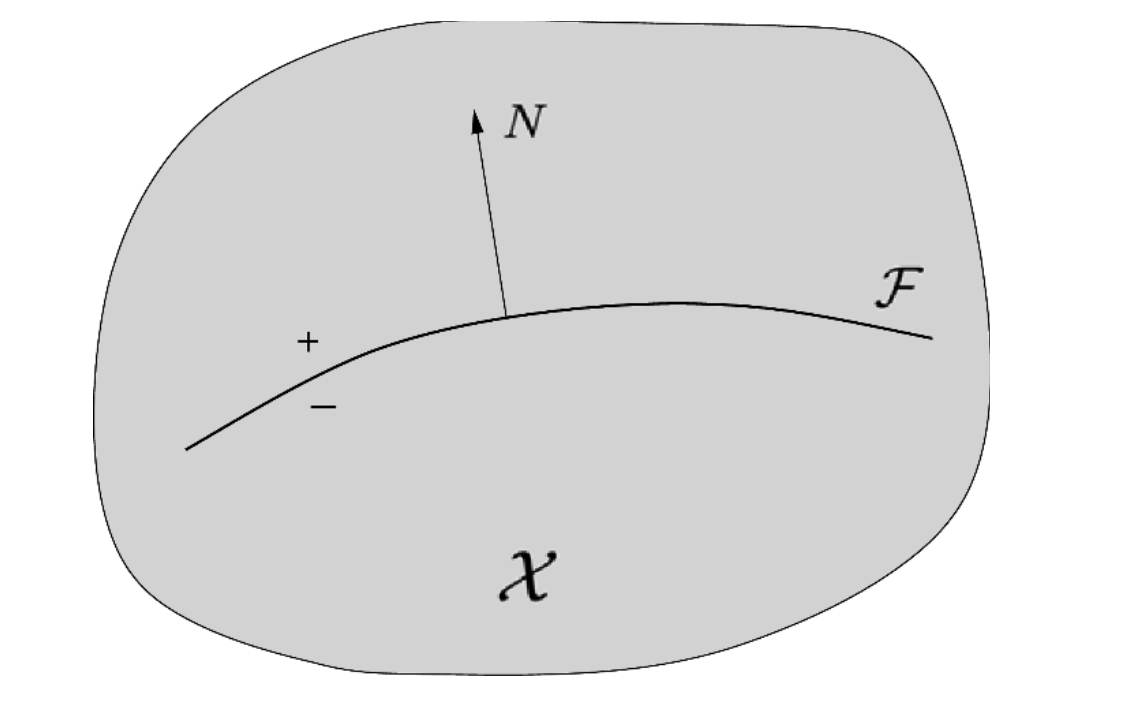
\includegraphics[width=0.6\textwidth]{../../image/ch01-fig06-01.png}
\caption{余维 $1$ 阵面 $\mathscr{F}$、法向 $N$ 与两侧 $+$、$-$。}\label{figure:ch01-front}
\end{figure}

$U$ 是平衡律方程组\cref{align:ch01-closed-system} 在 $\mathscr{X}$ 上的一个（一般为弱的）解，在 $\mathscr{X}\setminus\mathscr{F}$ 上连续可微，但允许在 $\mathscr{F}$ 上奇异。特别地，\cref{align:ch01-closed-system} 对任意 $X\in\mathscr{X}\setminus\mathscr{F}$ 成立；见\cref{figure:ch01-front}。

首先考虑 $\mathscr{F}$ 是\emph{弱阵面}（weak front）的情形，即 $U$ 在 $\mathscr{X}$ 上 Lipschitz 连续，而当从两侧趋近 $\mathscr{F}$ 时，$U$ 的梯度达到不同极限 $\operatorname{grad}^{-}U$、$\operatorname{grad}^{+}U$。于是 $\llbracket\operatorname{grad}U\rrbracket=\operatorname{grad}^{+}U-\operatorname{grad}^{-}U$ 是 $\operatorname{grad}U$ 跨过 $\mathscr{F}$ 的跃度。由于 $U$ 连续，$U$ 的切向导数不能跨过 $\mathscr{F}$ 跳跃，因而 $\llbracket\operatorname{grad}U\rrbracket=\llbracket\partial U/\partial N\rrbracket N^{\top}$，其中 $\llbracket\partial U/\partial N\rrbracket$ 表示法向导数 $\partial U/\partial N$ 跨过 $\mathscr{F}$ 的跃度。因此，在任一点 $X\in\mathscr{F}$ 处取\cref{align:ch01-closed-system} 跨过 $\mathscr{F}$ 的跃度，得到关于 $\llbracket\partial U/\partial N\rrbracket$ 的如下条件：
\begin{align}
\mathsf{D}\bigl[G(U(X),X)N\bigr]\left[\left[\frac{\partial U}{\partial N}\right]\right]=0.\label{align:ch01-weak-front-jump}
\end{align}

其次假设 $\mathscr{F}$ 是\emph{激波阵面}（shock front），即当从两侧趋近 $\mathscr{F}$ 时，$U$ 达到不同极限 $U_{-},U_{+}$，从而跨过 $\mathscr{F}$ 经历跃度 $\llbracket U\rrbracket=U_{+}-U_{-}$。$U_{-}$ 与 $U_{+}$ 都是 $\mathscr{F}$ 上的连续函数。由于 $U$ 是\cref{align:ch01-closed-system} 的（弱）解，对任意 $\varphi\in C_{0}^{\infty}(\mathscr{X})$ 可写\cref{align:ch01-weak-system}。在\cref{align:ch01-weak-system} 中，$\mathscr{X}$ 上的积分可换为 $\mathscr{X}\setminus\mathscr{F}$ 上的积分。由于 $U$ 在 $\mathscr{X}\setminus\mathscr{F}$ 上 $C^{1}$，可在\cref{align:ch01-weak-system} 中分部积分。利用 $\varphi$ 在 $\mathscr{X}$ 中具紧支集且\cref{align:ch01-closed-system} 对任意 $X\in\mathscr{X}\setminus\mathscr{F}$ 成立，得到
\begin{align}
\int_{\mathscr{F}}\varphi(X)\bigl[G(U_{+},X)-G(U_{-},X)\bigr]N\,\mathrm{d}\mathscr{H}^{k-1}(X)=0,\label{align:ch01-shock-integral}
\end{align}
由此推出在激波阵面 $\mathscr{F}$ 的每一点 $X$ 处必须满足如下\emph{跃度条件}：
\begin{align}
\bigl[G(U_{+},X)-G(U_{-},X)\bigr]N=0.\label{align:ch01-Rankine-Hugoniot}
\end{align}
注意\cref{align:ch01-Rankine-Hugoniot} 可改写为
\begin{align}
\left\{\int_{0}^{1}\mathsf{D}\bigl[G(\tau U_{+}+(1-\tau)U_{-},X)N\bigr]\,\mathrm{d}\tau\right\}\llbracket U\rrbracket=0.\label{align:ch01-shock-averaged}
\end{align}
将\cref{align:ch01-shock-averaged} 与\cref{align:ch01-weak-front-jump} 比较，我们得出结论：弱阵面可视为“无穷小”强度的激波阵面，$|\llbracket U\rrbracket|$ 消失性地小。

对每个 $U\in\mathcal{O}$ 与 $X\in\mathscr{X}$，我们联系以 variety
\begin{align}
\mathscr{V}(U,X)=\{(N,V)\in\mathbb{S}^{k-1}\times\mathbb{R}^{n}:\mathsf{D}[G(U,X)N]V=0\}.\label{align:ch01-variety}
\end{align}
\cref{align:ch01-closed-system} 的解所能支撑的小强度弱阵面与激波阵面的数目取决于 $\mathscr{V}$ 的大小。在极端情形：对所有 $(U,X)$，$\mathscr{V}(U,X)$ 在 $\mathbb{R}^{n}$ 上的投影仅含向量 $V=0$，此时\cref{align:ch01-closed-system} 称为\emph{椭圆型}。于是平衡律方程组为椭圆型，当且仅当它不能支撑任何小强度的弱阵面或激波阵面。与椭圆性相对立的另一极端——即 $\mathscr{V}$ 达到最大可能尺寸——是\emph{双曲性}，它将在%

\cref{chapter:ch03-双曲平衡律方程组} 中引入。

\end{document}
